\documentclass[titlepage]{article}
\usepackage{float}
\usepackage{graphicx}
\graphicspath{ {./img/SystemRequirement} }
\usepackage[utf8]{inputenc}
\restylefloat{table}
\usepackage{longtable}
\usepackage{amssymb}
\usepackage{amstext}
\usepackage{amsthm}
\usepackage{amsmath}
\usepackage{enumerate}
\usepackage{fancyhdr}
\usepackage[margin=1in]{geometry}
\usepackage{graphicx}
\usepackage{extarrows}
\usepackage{setspace}
\usepackage{fullpage}
\usepackage{booktabs}
\usepackage{ulem}
\usepackage{tabularx}
\usepackage{makecell}
\usepackage{hyperref}
\usepackage[round]{natbib}
\usepackage[english]{babel}

\pagestyle{fancy}  
\setlength\parindent{0pt}
\renewcommand\headrulewidth{0.4pt}                                      
\renewcommand\footrulewidth{0.4pt}

\title{SE 4GB6: Draft System Requirements\\The Cut}
\author{Group 17\\\\
            Joseph Lu - luy89 \\
            Matthew Po - pom \\
            Stanley Liu  liuz23 \\
            Suhavi Sandhu - sandhs11
            }
\date{November 1, 2019}

% Setup fancyhdr package
\fancyhf{}
\fancyhfoffset{0em}
% Remove head rule
\renewcommand{\headrulewidth}{0pt}
\renewcommand{\footrulewidth}{0pt}
\fancyfoot[L]{Group17 - The Cut}
\fancyfoot[C]{Page \thepage}
\fancyfoot[R]{Revision 1.0}

\begin{document}

\maketitle
\tableofcontents

\newpage
\section{Revision}

\begin{table}[H]
    \centering

    \begin{tabularx}{\textwidth}{|c|c|c|X|}
        \hline
        Date & Revision Number & Authors & Comments \\ 
        \hline
        October 29, 2019 & 0 & \makecell{Matthew Po\\Suhavi Sandhu\\Stanley Liu\\Joseph Lu} & -\\ 
        \hline
        January 7, 2020 & 1 & \makecell{Matthew Po\\Suhavi Sandhu\\Stanley Liu\\Joseph Lu} & Modified Goals, Constants, Variables, and Non-Functional Requirements\\ 
        \hline
    \end{tabularx}
    \caption{Revision}
    \label{tab:Revision}
\end{table}

\newpage
% Document Purpose
\section{Document Purpose}
The purpose of this document is to outline the overall design, architecture, and ideas of our project and its requirements with respect to consumers. Our goal is to provide a clear understanding of our software product, its parameters, and the goal we wish to achieve.\\\\
In this document, we shall attempt to predict and sort out how we hope this product will be used in order to gain a better understanding of the project, outline concepts that will be developed, and document ideas that may be considered, but could also be discarded as the product develops. This document will also highlight the project’s target audience, predicted behaviour, constraints, as well as software requirements. 

\subsection{Scope}

\subsubsection{Project Purpose}
The purpose of our project is to provide our clients with an android application that can identify movies based on a set of video and audio input. The application will accept these parameters and return the movie title along with other metadata (cast, synopsis, genre, box office details, production company, etc) related to the film. 

\subsubsection{Goals}
\begin{table}[hbtp]
    \centering
    \begin{tabular}{|c|c|}
        \hline
         & GOALS (not in any particular order)\\
         \hline
         1 & Return a response within 10 seconds\\
         \hline
         2 & Process uploaded videos\\
         \hline
         3 & Recognize foreign films\\
         \hline
    \end{tabular}
    \caption{Project Goals}
\end{table}

\begin{enumerate}
    \item Return a response within 10 seconds
    \begin{itemize}
        \item the application will respond after a video has been uploaded
        \item the response may be a list of movies within 10 seconds or a notification informing the user the processing is taking longer than expected
        \item each movie will include meta data and confidence percentages
    \end{itemize}
    
    \item process uploaded videos
    \begin{itemize}
        \item The application can record videos straight from the user's phone camera and be uploaded for processing
    \end{itemize}
    
    \item Recognize foreign films
    \begin{itemize}
        \item The movies recognized by the application extends beyond Hollywood films
        \item Chinese, Bollywood, Indie
    \end{itemize}
\end{enumerate}

\subsubsection{Project Scope}
The scope of the project is to be able to identify movies from short video clips. The development team will be focusing on Hollywood movies. Users will be able to input a video clip and the system will give a list of movies with confidence percentages. The scope of the information that will be retrieved is meta data such as actors, release date and description.

\subsection{Intended Audience / Stakeholders}

\subsubsection{Intended Audience}
\begin{itemize}
    \item Mobile Device Users
\end{itemize}

\subsubsection{Stakeholders}
\begin{itemize}
    \item Dr. Alan Wassyng
    \item Nicholas Annable
    \item Curtis Milo
    \item Rohan Patel
    \item Tim Tomashevski
\end{itemize}

% \subsection{Intended Use}
% The application will be used in a casual setting. The user will open the application and record a video through the camera, After 10 seconds, a list of movies and the confidence level for each movie is displayed. Clicking on each movie will show the movie metadata.

\newpage
% Overall System Design
\section{Overall System Design}

\subsection{Intended Functionality of System}
The main intended functionality of the system is to identify movies based on a set of video and audio input. It is aimed for users who find out what movie is the video from.

\subsection{System Context}

\subsubsection{Context Diagram (Showing Boundaries)}
\begin{figure}[H]
    \centering
    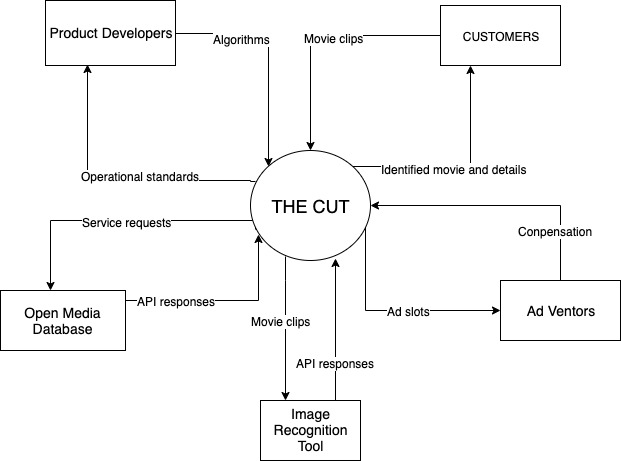
\includegraphics[width = 15cm]{img/SystemRequirement/contextDiagram.jpg}
    \caption{Context Diagram Showing Boundaries}
    \label{fig:Context}
\end{figure}

\subsection{Constraints}
\begin{table}[H]
    \centering
    \begin{tabular}{|c|l|}
        \hline
        \textbf{C2} & \textbf{Project must be finished within the academic year} \\
        \hline
        \textbf{Rationale} & The project must be submitted by the end of the academic year as per project requirements \\
        \hline
        \textbf{C1} & \textbf{Budget must be within \$300}\\
        \hline
        \textbf{Rationale} & 300 dollars has been set in line with other projects.\\
        \hline
    \end{tabular}
    \caption{Constraints}
    \label{tab:Constaints}
\end{table}

% System Features and Requirements
\section{System Features and Requirements}

\subsection{Functional Requirements}
\begin{table}[H]
    \centering
    \begin{tabularx}{\textwidth}{|c|X|} \hline
         & \textbf{Requirement} \\ \hline
        F1 & The Cut must be able to take movies with the smartphone camera. \\ \hline
        F2 & The Cut shall ask permission for User's camera,microphone, and WIFI \\ \hline
        F3 & The Cut shall display a List of movies with Confidence Percentages between 0\% and 100\% when input is processed\\ \hline
        F4 & The Cut shall inform the users if input was not processed \\ \hline
        F5 & The Cut shall display The Metadata of movies that have been distinguished. \\ \hline
        F6 & The Cut shall allow users to search through past movie searches \\ \hline
        F7 & The Cut shall be able to recognize foreign films \\ \hline
    \end{tabularx}
    \caption{Functional Requirements}
    \label{tab:Functional}
\end{table}

\subsection{Functional Requirements likely to change (nice-to-haves)}
\begin{table}[H]
    \centering
    \begin{tabularx}{\textwidth}{|c|X|} \hline
         & \textbf{Rationale} \\ \hline
        F4 & Subject to change, Scope not finalized \\ \hline
        F6 & Subject to change, Scope not finalized \\ \hline
        F7 & Subject to change, Scope not finalized \\ \hline
        F9 & Platform the application will be based on can change \\ \hline
    \end{tabularx}
    \caption{Functional Requirements likely to change}
    \label{tab:Functional_likely}
\end{table}

\subsection{Functional Requirements unlikely to change}
\begin{table}[H]
    \centering
    \begin{tabularx}{\textwidth}{|c|X|} \hline
         & \textbf{Rationale} \\ \hline
        F1 & Key Implementation \\ \hline
        F2 & Software Policy \\ \hline
        F3 & Key Implementation\\ \hline
        F5 & Key Implementation \\ \hline
    \end{tabularx}
    \caption{Functional Requirements unlikely to change}
    \label{tab:Functional_unlikely}
\end{table}

\subsection{Non-functional Requirements}
\subsubsection{Look and Feel Requirements}
\begin{table}[H]
    \centering
    \begin{tabularx}{\textwidth}{|c|X|} \hline
        NF1 & The Cut shall be clear which state the user is in \\ \hline
        NF2 & The Cut must hide the states that the user isn't in \\ \hline
        NF3 & The Cut must display non-offensive and appealing colours \\ \hline
    \end{tabularx}
    \caption{Look and feel requirements}
    \label{tab:NonFunctional-look and feel}
\end{table}

\subsubsection{Ease of Use Requirements}
\begin{table}[H]
    \centering
    \begin{tabularx}{\textwidth}{|c|X|} \hline
        NF4 & The Cut must make movies easy to read and interact with \\ \hline
    \end{tabularx}
    \caption{Ease of use requirements}
    \label{tab:NonFunctional-ease of use}
\end{table}

\subsubsection{Performance Requirements}
\begin{table}[H]
    \centering
    \begin{tabularx}{\textwidth}{|c|X|} \hline
        NF5 & The Cut must be able to distinguish movies within 10 seconds \\ \hline
        NF6 & The system should be able to store up to 60 seconds of a movie clip \\ \hline
        NF7 & The amount of time required for the clip to be processed by both audio and image processing modules should be less than 120 seconds \\ \hline
        Rationale & This is the estimated time of processing taking account of the time to upload images/audios and running analysis \\ \hline
    \end{tabularx}
    \caption{Performance requirements}
    \label{tab:NonFunctional-performance}
\end{table}

\subsubsection{Compatibility Requirements}
\begin{table}[H]
    \centering
    \begin{tabularx}{\textwidth}{|c|X|} \hline
        NF8 & The Cut shall be able to run on Android 8.0 and higher \\ \hline
        Rationale & Android 8.0 was initially released in August 2017, and is still used by a lot of people \\ \hline
    \end{tabularx}
    \caption{Compatibility requirements}
    \label{tab:NonFunctional-compatibility}
\end{table}

\subsubsection{Reliability Requirements}
\begin{table}[H]
    \centering
    \begin{tabularx}{\textwidth}{|c|X|} \hline
        NF9 & Under normal usage conditions, the application should not experience critical failure 90 percent of the time \\ \hline
        Rationale & This is the estimated percentage of the time the application is functioning correctly \\ \hline
    \end{tabularx}
    \caption{Reliability requirements}
    \label{tab:NonFunctional-reliability}
\end{table}

\subsubsection{Maintainability Requirements}
\begin{table}[H]
    \centering
    \begin{tabularx}{\textwidth}{|c|X|} \hline
        NF10 & There should be an 80 percent chance that a bug or the server to be fixed in 12 hours \\ \hline
        Rationale & This is the estimated percentage of chance that the developer is able to fix the issue within 12 hours \\ \hline
    \end{tabularx}
    \caption{Maintainability requirements}
    \label{tab:NonFunctional-Maintainability}
\end{table}

\subsubsection{Availability Requirements}
\begin{table}[H]
    \centering
    \begin{tabularx}{\textwidth}{|c|X|} \hline
        NF11 & The Cut should be available to use 99.5 percent of the time during a month \\ \hline
        Rationale & Assuming there is server maintenance once every two weeks, 2 hours per maintenance, the application should be available 99.5 percent of the time during a month \\ \hline
    \end{tabularx}
    \caption{Availability requirements}
    \label{tab:NonFunctional-Availability}
\end{table}

\subsubsection{Security Requirements}
\begin{table}[H]
    \centering
    \begin{tabularx}{\textwidth}{|c|X|} \hline
        NF12 & The Cut should not be able to access any personal data on the device \\ \hline
    \end{tabularx}
    \caption{Security requirements}
    \label{tab:NonFunctional-Security}
\end{table}

\subsection{Constants}
\begin{enumerate}
    \item \textbf{Seconds} - The amount of time measured for each video submission as well as response from the application.
\end{enumerate}

\subsection{Variables}
\begin{table}[H]
    \centering
    \begin{tabularx}{\textwidth}{|c|X|c|c|c|}
        \hline
        \textbf{Name} & \textbf{Description} & \textbf{Type} & \textbf{Units} & \textbf{Range}\\
        \hline
        InputClipLength & Length of video submission & Controlled & Seconds & [10,60] \\
        \hline
        UploadAttempt & The number of application attempts to upload a video file to the server. & Monitored & Integer & [0,5] \\
        \hline
        ApplicationWaitTime & Time constraint for application to respond to a request over a network. Should processing take longer than this, the application will relinquish control back to the user and notify them once the results have been processed. & Monitored & Seconds & (0,10] \\
        \hline
        ProcessTime & Amount of time required for video to be processed by both audio and image processing modules. Should processing take longer than the allotted time, it is considered to be failed. & Monitored & Seconds & (0, 120] \\
        \hline
    \end{tabularx}
    \caption{Caption}
    \label{tab:Variables}
\end{table}

\newpage
% System Behaviour
\section{System Behaviour}

\subsection{Behaviour Overview}
The behaviour of the system acts like the diagram in section 4.2. The system waits for the input of user. If there is an valid input(video/audio), the video is being processed; else, the system asks for a valid input. Then, if the movie is identified, report to the user; else, tell the user that it is not identified.


\subsection{Diagrams for Functional Decomposition}
\begin{figure}[H]
    \centering
    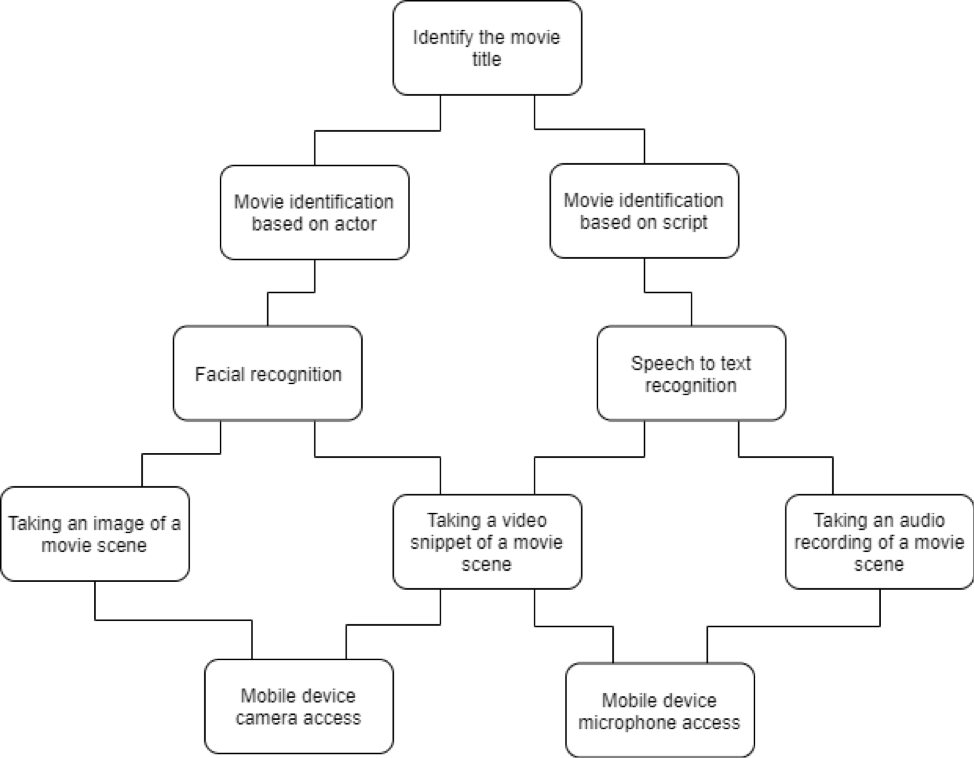
\includegraphics[width = 15cm]{img/SystemRequirement/fd.png}
    \caption{Functional Decomposition Diagram}
    \label{fig:Functional_Decomposition}
\end{figure}

\subsection{Required Behaviour Description}
\begin{figure}[H]
    \centering
    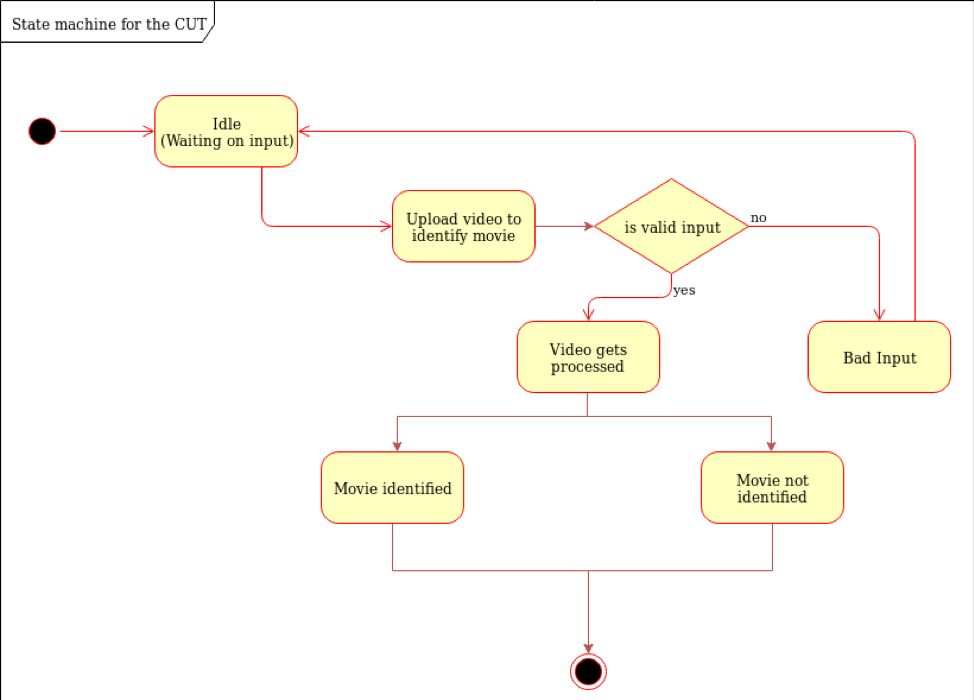
\includegraphics[width = 15cm]{img/SystemRequirement/stateMachine.png}
    \caption{State Machine Diagram}
    \label{fig:State_Machine}
\end{figure}
\begin{table}[h!]
    \centering
    \begin{tabularx}{\textwidth}{|l|X|}
    \hline
    \textbf {State}  & \textbf {Description} \\
    \hline
    Idle & The system is open and ready to accept video input\\
    \hline
    Record Video & The user records a video using their mobile device.\\
    \hline
    Upload video & The application attempts to upload a video to the server for processing. A maximum of \hyperref[tab:Variables]{\textbf{UploadAttempts}} is allocated before considering the state a failure.\\
    \hline
    Video Processing & The video is processed by modules.\\
    \hline
    Return Result & The video has been processed and is either identified (success) or not identified (failed) and the execution of the system ends. The result is returned to the user.\\
    \hline
    \end{tabularx}
    \caption{Required Behaviour Description}
    \label{tab:States}
\end{table}

\subsection{Normal Behaviour}
Under normal operating conditions, the application shall be able to run on a mobile device that supports Android 10 (https://developer.android.com/about/versions/10/features). The application shall have access to the mobile devices’ camera and microphone hardware to have the ability to take image, video, and/or audio snippets. The mobile device will be connected to the internet for quick results. 

\subsection{Undesired Event Handling}
\begin{enumerate}
    \item Application unexpectedly crashes during identification process/cell phone unexpectedly turns off
        \begin{itemize}
        \item The system will save the latest uploaded movie clip, so next time the user will not have to upload the clip again
        \item The system will automatically run a troubleshooting test to check the storage, memory usage, battery level the cell phone
        \end{itemize}
   \item Identification process takes too long due to weak internet signal or slow internet connection
        \begin{itemize}
        \item The system will notify the user about the internet latency and suggest the user to run the application under WIFI connection
        \end{itemize}
    \item Input clip length is too short to provide sufficient information for the application to identify the movie
        \begin{itemize}
        \item The system will notify the user to upload a longer clip, or film the video longer
        \end{itemize}
\end{enumerate}


\end{document}
